\documentclass[a4paper,11pt]{article}

%% Language and font encodings
\usepackage[english]{babel}
\usepackage[utf8x]{inputenc}
\usepackage[T1]{fontenc}
\usepackage{subcaption}

%% Sets page size and margins
\usepackage[a4paper,top=3cm,bottom=2cm,left=3cm,right=3cm,marginparwidth=1.75cm]{geometry}

%% Useful packages
\usepackage{amsmath}
\usepackage{graphicx}
\usepackage[colorinlistoftodos]{todonotes}
\usepackage[colorlinks=true, allcolors=blue]{hyperref}




\begin{document}

\vspace*{13mm}
\begin{center}
\rule[0.5ex]{\linewidth}{2pt}\vspace*{-\baselineskip}\vspace*{3.2pt}
\rule[0.5ex]{\linewidth}{1pt}\\[\baselineskip]
{\Huge Robust Augmented Reality using RGB-D SLAM}\\[4mm]

\rule[0.5ex]{\linewidth}{1pt}\vspace*{-\baselineskip}\vspace{3.2pt}
\rule[0.5ex]{\linewidth}{2pt}\\
\vspace{6.5mm}
{\large By}\\
\vspace{6.5mm}
{\large\textsc{Ze Zhang}}\\
\vspace{11mm}

\includegraphics[scale=0.6]{bristolcrest_colour}\\
\vspace{6mm}
{\large Department of Engineering Mathematics\\
\textsc{University of Bristol}}\\
\vspace{11mm}
\begin{minipage}{10cm}

\end{minipage}\\
\vspace{9mm}
{\large\textsc{31 March 2017}}
\vspace{12mm}
\end{center}

\newpage
\section{Aims and Objectives}
\subsection{Aims}
This project will study how to develop a robust Augmented Reality (AR) system based on RGB-D SLAM system. This AR system will use the accurate 3D model which is generated by SLAM system, so it is more robust and accurate than most other AR system. 
\subsection{Objectives}
\begin{itemize}
\item Study RGB-D SLAM system.
\item Connect new RGB-D sensor with SLAM system.
\item Using SLAM system to contrast 3D model.
\item Using AR software to create virtual character.
\item Apply AR system in google map if time permits.
\end{itemize}


\section{Motivation}
AR and VR are two hot concept today, prevalent people also know them as VR film and AR game. I know AR because of the famous mobile game pokemon go which is showed in figure 1a. Then I find another AR app called SekaiCamera which is developed by Japanese company Tonchidot in figure 1b. It can add comments on object which is captured by your phone camera. I think AR is more useful than VR because it adds information on real scene instead of create a new scene. However, pokemon go and SekaiCamera are simple AR systems which only use 2D image and GPS. I want to develop a more robust AR system based on accurate 3D model which is provided by RGB-D SLAM system.

\begin{figure}[!htp]
		\centering
		\begin{subfigure}{.5\textwidth}
			\centering
			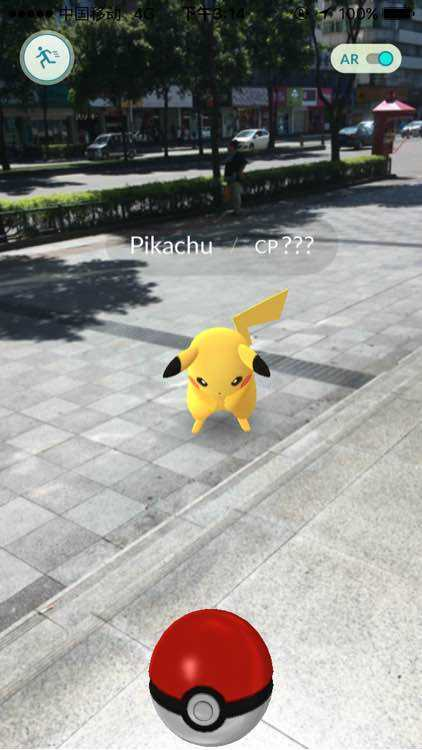
\includegraphics[width=0.7\linewidth]{1.jpg}
			\caption{pokemon go}
		
		\end{subfigure}%
		\begin{subfigure}{.5\textwidth}
			\centering
			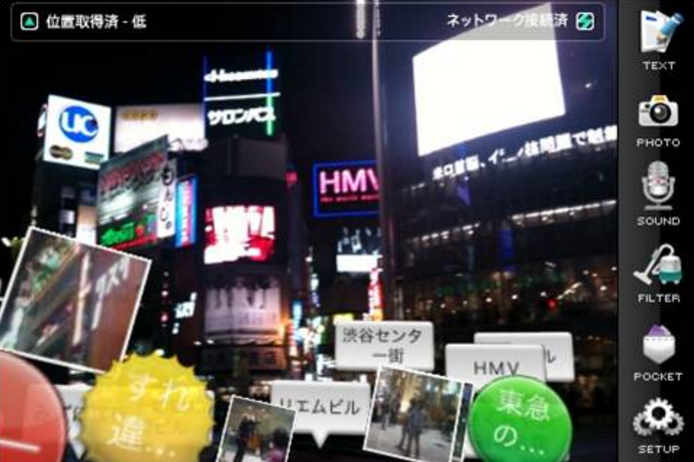
\includegraphics[width=1.2\linewidth]{2.png}
			\caption{SekaiCamera}
			
		\end{subfigure}
		\caption{AR system}
		\label{fig:fig1}
	\end{figure}

\end{document}
